\section{\name solution}
\label{sec:algorithm}
We build upon the ideas in \S\ref{sec:insights} to present the techniques in our solution, \name, to reduce  the cost of profiling for online adaptation of configurations.%, by leveraging the temporal and spatial correlations above.

{\name}'s solution relies on periodically profiling, or ``re-profiling'' the video pipeline. Video workloads are typically ``non-stationary'', \ie both the characteristics of the video as well as the pipeline tend to change over time. This makes model-based approaches (\eg Bayesian optimization, multi-armed bandits, etc.) either too expensive for real-time adaptation or unsuited because of their assumption of a stationary environment (despite their successful use in recent systems~\cite{ernest,cherrypick,amazon-bandit}).

%At a high level, \name leverages the tendency of good configurations to persist over time (\S\ref{subsec:temporal-impl}), and to perform well across similar video feeds (\S\ref{subsec:spatial-impl}), to greatly reduce the re-profiling cost. Nevertheless, some amount of periodic re-profiling is unavoidable due to the dynamic (non-stationary) nature of video analytics pipelines, as we made the case for in \S\ref{sec:potential}. This non-stationarity in the face of real-time videos makes traditional modeling approaches (\eg Bayesian optimization, multi-armed bandits, etc.) too expensive, despite their successful use in several recent (but stationary) systems scenarios~\cite{ernest,cherrypick,amazon-bandit}. We compare \name to these works in \S\ref{sec:related}. Instead, 

\name uses a solution inspired by greedy hill climbing that exploits the independence and structure of the \nn configuration knobs to reduce the search space from exponential to linear (\S\ref{subsec:profile-alg}). Using this profiling method, it learns the properties of configurations over time (\S\ref{subsec:temporal-impl}) and amortizes the cost of profiling across multiple cameras (\S\ref{subsec:spatial-impl}). 

\subsection{Overview}

\begin{figure}[t!]
\centering
%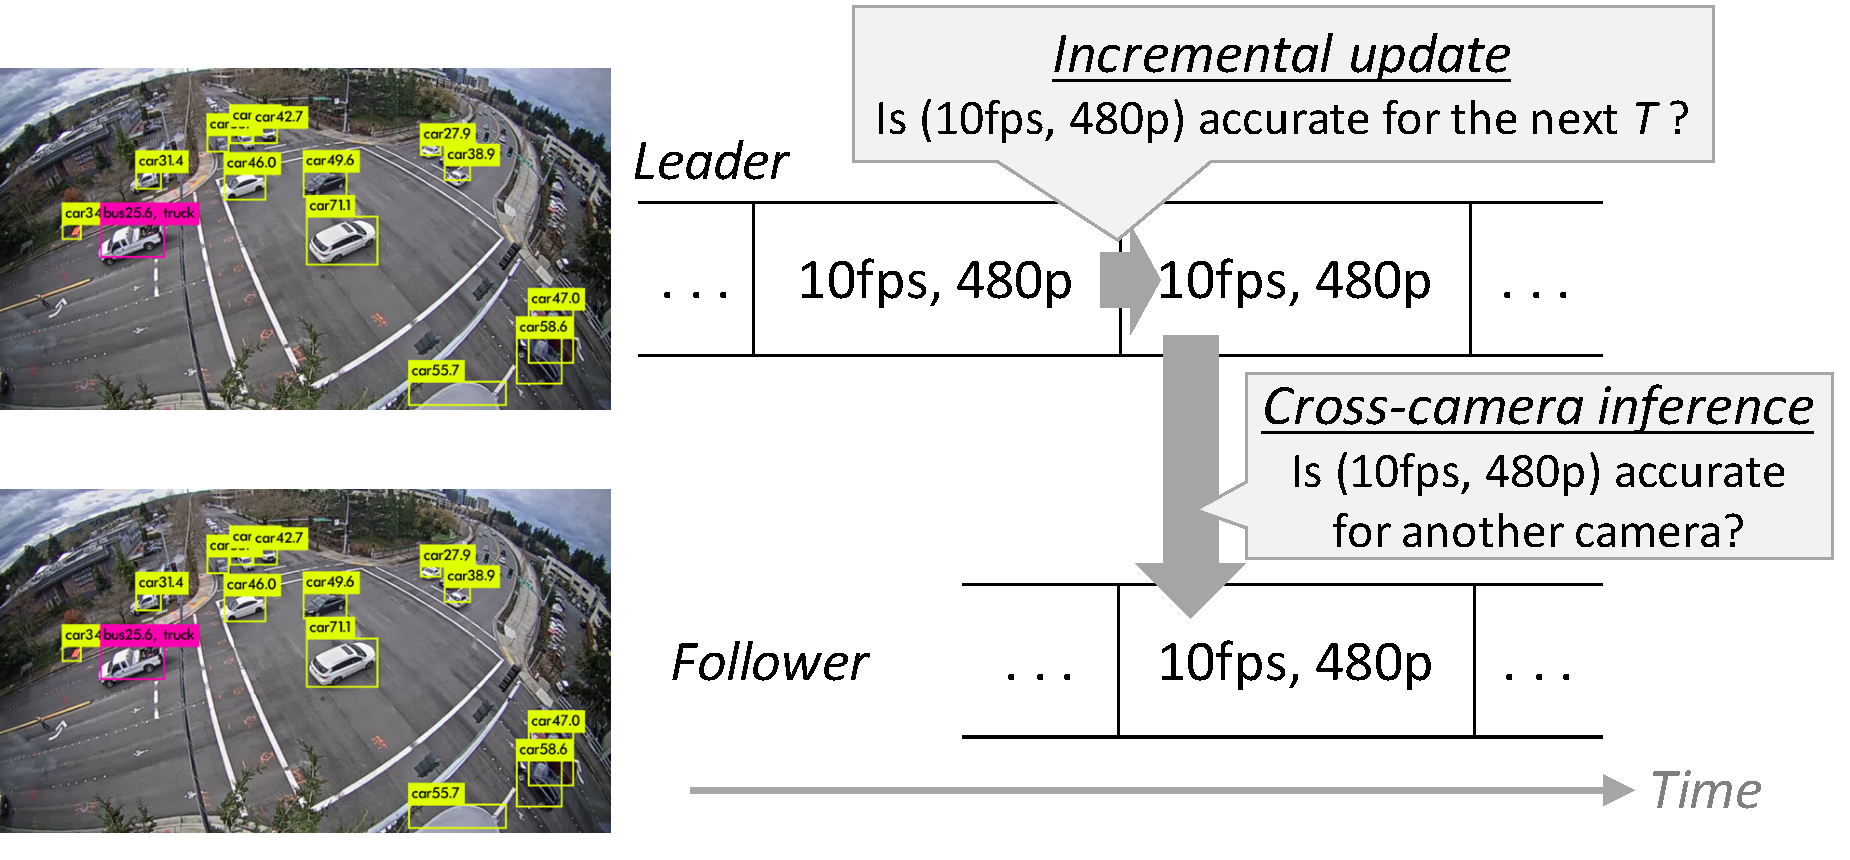
\includegraphics[width=0.5\textwidth]{PaperFigures/Workflow.pdf}
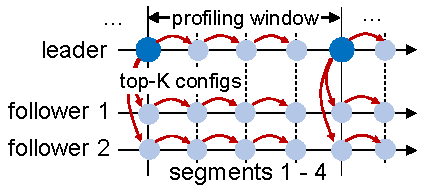
\includegraphics[width=0.4\textwidth]{figures/profiling_cropped.pdf}
\vspace{-0.2cm}
\tightcaption{
The horizontal lines represent video feeds generated by three cameras over time (one leader, two followers). The solid vertical lines delineate profiling windows and the dashed vertical delineate segments. The blue circles represent profiling (\S\ref{subsec:profile-alg}); bigger dark circles represent full profiling of the whole configuration space, which yields the top-$k$ most promising configurations from the leader. The red arrows show the propagation of the top-$k$ configs both temporally (to segments on the same camera, \S\ref{subsec:temporal-impl}), and spatially (to segments on the follower cameras, \S\ref{subsec:spatial-impl}). 
%The small light circles represent profiling that only considers the top-K configurations.
%Example of how a good configuration from one video segment
%is carried over to other segments, across time (right arrow) and space (down arrow).
}
\label{fig:workflow}
\end{figure}

Figure~\ref{fig:workflow} gives an overview of \name's techniques. A "leader" video is profiled at the start of a "profiling window" and a good (top-$k$) set of configurations is found. This set is shared among "follower" videos who are spatially similar to the leader. Both the leader and followers can then restrict their search to these top-$k$ configurations when choosing configurations over time, until the start of the next profiling window (when a new top-$k$ set will be obtained from the leader). All of these terms are defined in the subsequent sections.

%configuration is applied to the next segment of the leader's video (Algorithm~\ref{alg:temporal}) and the next segment of a follower's video (Algorithm~\ref{alg:spatial}). Only the initial profiling of the leader is expensive; the application to subsequent segments (at both the leader and follower) only searches a small, top-$k$ set of configurations.


\subsection{Temporal incremental updates}
\label{subsec:temporal-impl}

\ga{The notation $T$ below conflicts with Section 3.} \sid{I will make this consistent, hopefully allowing us to remove R}

\begin{algorithm}[t!]
    % \small
	\DontPrintSemicolon
    \SetKwFunction{ProcessWindowTemporal}{UpdateWindowT}
    \SetKwFunction{Profile}{Profile}
    \SetKwProg{Fn}{Function}{:}{}
	\KwIn{$W_{i,l}$: the $l^\textrm{th}$ profile window of the
	$i^\textrm{th}$ video; $C$: set of all configurations under consideration}
	\KwOut{Configuration $\hat{c}_{i,j}$ for each segment $S_{i,j}$.}
    \Fn{\ProcessWindowTemporal{$W_{i,l},C$}}{
        $Result\leftarrow\emptyset$\\
        %\tcc{\small{Profile first segment on full config space, then reuse promising ones}}
        $C_l^{promising}\leftarrow$ \Profile{$S_{i,wl},C,k$}\\
        $Result.add(\hat{c}_{i,0}, C_l^{promising}[0])$\\
        \ForEach{$j=wl+1,\dots,w(l+1)-1$}{
            $C\leftarrow$\Profile{$S_{i,j},C_l^{promising},1$}\\
            $Result.add(\hat{c}_{i,j}, C[0])$\\
        }
        \Return{$Result$}
    }
	\caption{Temporal updates take promising configurations from the first segment of a profiling window and apply them to subsequent segments in the window.}
	\label{alg:temporal}
\end{algorithm}

{\name} periodically records and profiles the video pipeline using an interval we refer to as the {\em profiling window}. 
%In each window, it records and profiles a video feed of length $R$. 
Each window is split into smaller {\em segments}, each of which is a contiguous set of frames spanning a $T$-second interval (by default, $T = 4$). We leverage temporal persistence (\S\ref{subsec:temporal}) by not profiling all the segments in a profiling window. Instead, we re-profile the configuration space on only the first segment of the profiling window. It uses the results from this first segment to obtain a small list of the top-$k$ most promising configurations (\ie the least expensive $k$ configurations that meet the accuracy threshold), and then profiles only the top-$k$ configurations on the remaining segments to find the best one. When profiling a configuration on a segment, we do not evaluate every frame of the segment---this would defeat the purpose of finding a low-cost configuration. Instead, we profile the first $t$ seconds (by default, $t = 1$) and use the best configuration found on the remaining $T-t$ seconds. \ga{How do we combine results across the remaining segments?}

%The first technique in \name exploits the temporal persistence of \nn performance (\S\ref{subsec:temporal}) to incrementally update the current \nn configuration. See Algorithm~\ref{alg:temporal}.

Algorithm~\ref{alg:temporal} lists the steps taken in each profiling window given a video stream  $i$. For the $i^\textrm{th}$ video, we use $S_{i,j}$ to denote the $j^\textrm{th}$ segment and $W_{i,l}$
to denote the $l^\textrm{th}$ profiling window, which is a list of $w$ consecutive segments 
$(S_{i,wl},\dots,S_{i,w(l+1)-1})$. Line 3 in the algorithm picks the top-$k$ configurations from the first segment, and lines 5-7 use the top-$k$ set to profile the remaining segments. Both these steps use the \Profile method, which we will cover in \S\ref{subsec:profile-alg}.

%\name splits each video feed into {\em segments}, each of which is a list of frames spanning a small $T$-second time interval (by default, $T=4$). For the $i^\textrm{th}$ video, we use $S_{i,j}$ to denote the $j^\textrm{th}$ segment and $W_{i,l}$ to denote the $l^\textrm{th}$ {\em profiling window}, which is a list of $w$ consecutive segments $(S_{i,wl},\dots,S_{i,w(l+1)-1})$. Due to its temporal persistence, the \nn  configuration does not need to be re-profiled every segment. Instead, \name re-profiles the configuration space once per profiling window. It uses the first segment of each profiling window to profile the full input configuration space, obtaining a small list of the top-$k$ most promising configurations (line~3). Then, for each remaining segment in the profiling window, it profiles only the top-$k$ configurations to find the best one (line~5-7).

There is an extension to the algorithm that learns across profiling windows to discard certain configurations and reduce the cost of profiling even the first segment. First, we discard configurations that are consistently bad (in the bottom-most 10\% in their accuracy). Second, we identify values of the knobs beyond which the accuracy of configurations plateau, and save on profiling beyond these plateau-values. %even for the first segment, we use only the union of the sets of top-$k$ configurations from the past few profiling windows.
Since our environment is non-stationary, we randomly but infrequently explore the discarded configurations in case they become good again. This extension is currently not used in our experiments.

\subsection{Spatial cross-video inference}
\label{subsec:spatial-impl}

\begin{algorithm}[t!]
    % \small
	\DontPrintSemicolon
    \SetKwFunction{CrossCamera}{CrossVideo}
    \SetKwFunction{GroupCameras}{GroupVideos}
    \SetKwFunction{ProcessWindowSpatial}{UpdateWindowS}
    \SetKwFunction{Profile}{Profile}
    \SetKwProg{Fn}{Function}{:}{}
	\KwIn{$G$: a list of all video feeds, $C$: set of all configurations under consideration}
	\KwOut{Configuration $\hat{c}_{i,j}$ for each segment $S_{i,j}$.}
    \Fn{\ProcessWindowSpatial{$l,G,C$}}{
        $Result\leftarrow \emptyset$\\
        $i\leftarrow G[0]$\\
        $Result.add(\ProcessWindowTemporal{$W_{i,l},C$})$\\
        $C_l^{promising}\leftarrow$ (returned by \Profile in line 4)\\ %\Profile{$S_{i,wl},C,k$}\\
        \ForEach{$i'\in G\setminus{i}$}{
            $Result.add(\ProcessWindowTemporal{$W_{i',l},C_l^{promising}$})$\\
        }
        \Return{$Result$}
    }
	\caption{Spatial updates take promising configurations profiled from one video and apply them to all other videos in the same related group.}
	\label{alg:spatial}
\end{algorithm}

In each profiling window, \name leverages spatial
similarities in \nn performance (\S\ref{subsec:spatial}) 
to amortize the cost of profiling across multiple video feeds. See 
Algorithm~\ref{alg:spatial}.

The ability to take good configurations profiled on one video stream and apply them 
to other video streams offers huge potential savings. Let $P$ be the cost of profiling a video segment on the full
configuration space ($C$), $p \ll P$ the cost of profiling only the top-$k$ most promising
configurations from a reference video ($C^{promising}$), and suppose there are $V$ videos in total.
If the videos are spatially unrelated \ga{As in?}, the cost of profiling them is $P\cdot V$ in
every profiling window. On the other hand, if the videos show spatial similarity, 
the cost reduces to $P + p(V-1)$, a savings that grows with the number of videos
$V$.

Algorithm~\ref{alg:spatial} takes a group of {\em related} video streams $G$ as input, and only profiles the first video (referred to as the ``leader'') on the full configuration space (lines~3-5). We discuss how we group the set of related videos shortly. The call to {\tt Update\sep WindowT} assigns a configuration to each segment of the window using the temporal update technique from \S\ref{subsec:temporal-impl}. 
%(Note that line 5 is technically redundant since it is already computed by the call on line 4, but %we include it here for clarity. \ga{Remove the line and just say the call in line 4 already calls %the \Profile method?}) 
For all remaining videos (the ``followers''), the call to {\tt Update\sep WindowT} only receives the most promising configurations from the first video as input (line~7), thus significantly reducing the search space.

There is an extension to the algorithm for when we pass the top-$k$ configurations from the leader to the followers. We have observed in practice that it is beneficial to include not only the current set of top-$k$ configurations but also those from the past few profiling windows. In other words, we sample from $\cup_{l\in \mathbb{W}}~C_l^{promising}$ to obtain the $k$ configurations, where $\mathbb{W}$ is the set of profiling windows in the past. This extension is currently not used in our experiments.

%\sid{Where to put below; also it needs cleaning/trimming. Come up with a term to describe the
%spatial window.}
%The actual algorithm we implement is slightly more complicated, in that it retains
%$C_l^{promising}$ 
%over multiple profiling windows in the recent past, addressing the reality that related videos may share optimal configurations from a larger time span than just a single profiling window. We call this time span the {\em spatial window}.  
%In other words, the set $C^{promising}$ of video $i$ in a given profiling window may not yield good %accuracy on a camera $j$ in that same window,
%but $C^{promising}$ from one of $i$'s previous profiling windows may do the trick. 
%For example, consider two traffic cameras that are separated by a block: although they may not see the same flow of traffic at the same instant in time, they will see very similar flows across longer (\eg several minute) time intervals. Thus, we modify Algorithm~\ref{alg:spatial} to sample configurations from the union $\cup_{l\in \mathbb{W}}~C_l^{promising}$, where $\mathbb{W}$ is the set of profiling windows spanning the most recent spatial window.

\noindent{\bf Grouping related videos:} %It remains to define how video feeds are grouped in the first place. For this, we reuse ideas from our existing algorithms. Since the correlations we exploit between videos are defined by the accuracy of running \nn configurations on them, we use this accuracy to perform the grouping. 
We group video feeds by exploiting the correlation between configurations on the accuracy of their output on different feeds; these accuracies are comparable across feeds since they are running the same pipeline. The grouping of video feeds is offline and done relatively infrequently (say, once every few hours).

The grouping algorithm starts with a randomly chosen configuration and profiles all videos on it, then uses the accuracy results to create an initial grouping using a simplified, parameter-less version of k-means---essentially, sort the accuracies and bound the deviation from the minimum of a group. We repeat this process by using another randomly chosen configuration to subdivide the groups created by the previous round, and so on. This greedy refinement stops when enough configurations have been tested or the groups become too small. More sophisticated grouping algorithms are certainly possible and are deferred to future work; the focus of this paper is to demonstrate the feasibility and potential savings of grouping videos.

\sid{Junchen, is the above underspecified? I'm not sure how much detail we want to get into; I tried to hint that it is not the final grouping algorithm we hope to use.}

%\jc{add a paragraph on how to group video feeds.}

\subsection{Profiling a video segment}
\label{subsec:profile-alg}

%\mypara{Reducing profiling overhead}
Algorithm~\ref{alg:temporal} reduces the profiling cost from once per video segment 
per video feed to once per profiling window per video feed. Algorithm~\ref{alg:spatial} 
further reduces the profiling cost from once per profiling window per video feed to once per profiling window per video group. Although this is a substantial savings, even profiling  
once can be very costly. This is because the configuration space is
multi-dimensional, consisting of several knobs each taking one of several values,
yielding exponentially many possible configurations. Assuming $m$ knobs and (for simplicity)
$n$ values for each knob, an exhaustive search of this space would involve $\bigO(m^n)$ configurations.
Instead, \name leverages the empirically-driven assumption from \S\ref{subsec:independence} that the knobs of our \nn configurations can be treated independently. This allow us to use
a variant of {\em greedy hill climbing}, where each knob is tuned while all other knobs are held fixed, reducing the search space to $\bigO(mn)$. 
%We explain the choice of default values further below.

% that the relationship between each knob's value and inference 
% accuracy is independent to the setting on other knobs. 
% For instance, if 5fps is the least frame rate to get an F1 
% score of 0.8 when the frame size is 960p, then 5fps will be the
% least frame rate to attain an F1 score of 0.8 when the frame size 
% is 480p.
% For instance, in pipeline $A$, the frame rate concerns the object
% moving speed, image sizes concerns the number of pixels to cover 
% each object of interest, and the object detection model depends on 
% whether the shape of an object can be expressed by the extracted 
% features.
% This allows us to profile knobs separately, and safely ignore the 
% combinational effects between knobs.

\begin{algorithm}[t!]
% \small
	\DontPrintSemicolon
    \SetKwFunction{Overall}{ConfigAdaptation}
    \SetKwFunction{ProfilingUnit}{Profile}
    \SetKwProg{Fn}{Function}{:}{}
	\KwIn{$S$: a segment; $C$: set of all configurations under consideration, $k$: number of top configurations to output.}
	\KwOut{A list of the top-$k$ best configurations in descending order.}
    \Fn{\ProfilingUnit{$S, C, k$}}{
        %$X\leftarrow$ the first $t$ seconds of $S$\\
        %$c^{default}=(v_1^{default},\dots,v_n^{default})$\\
        \tcc{\small{Profile one knob at a time}}
        $KnobValueToScore\leftarrow\emptyset$\\
        \ForEach{Knob $r$}{
            \ForEach{$v_r\in V_r$}{
                \tcc{\small{Change only knob $r$ to $v_r$, compare against golden config value $v_r^*$}}
                % $c(v_r)\leftarrow Replace(c^{default},r,v_r)$\\
                % $c(v_r^*)\leftarrow Replace(c^{default},r,v_r^*)$\\
                $c(v_r)\leftarrow (v_1^{*},\dots,v_r,\dots,v_n^{*})$\\
                $c^*\leftarrow (v_1^{*},\dots,v_r^*,\dots,v_n^{*})$\\
                \tcc{\small{Evaluate $c(v_r)$ using F1 metric}}
                $f\leftarrow Eval\_F1(S,c(v_r),c^*))$\\
                $KnobValueToScore(v_r)\leftarrow f$\\
            }
        }
        \tcc{\small{Overall accuracy is product of F1 scores across knobs}}
        $AccurateConfigs\leftarrow\{c\in C {|} \prod_{r}KnobValueToScore(v_r)\geq\alpha\}$\\
        Sort $AccurateConfigs$ by $c$'s resource consumption\\
        $AccurateConfigs\leftarrow$ top $k$ elements in $AccurateConfigs$\\
        \Return{$AccurateConfigs$}\\
    }
	\caption{Finds the top-$k$ best configurations for a segment efficiently by profiling each knob independently (a form of greedy hill climbing).}
	\label{alg:policy3}
\end{algorithm}

Algorithm~\ref{alg:policy3} shows how \name profiles each knob independently.
% For every $T$ seconds, it re-profiles and updates the 
% configurations on the frames in the first $t$ seconds.
For each value $v_r$ of knob $r$, we construct a configuration 
$c(v_r)$ with knob $r$ set to $v_r$ while all other knobs are set to their 
golden configuration (maximum) values. We compare $c(v_r)$ to the golden configuration $c^*$, which sets $r$ to its most expensive value (lines~5-7). 
%Note that $c(v_r^*)$ also leverages the independence assumption by setting all other knobs to their %default values; if we instead compared against the golden configuration across all knobs, this %would be incredibly more expensive. 
$Eval\_F1$ computes the average F1 score of a configuration $c$ with respect to
another configuration $c'$ over the frames in $S$, \ie $\frac{1}{|S|}\sum_{s\in S} F1(s,c,c')$. 
%(In practice, not all frames of $S$ need to be profiled---the first second or two suffices.)
%Let $Replace(C,r,v)$ denote the result of setting knob $r$ of $C$ 
%with $v$, and $F(X,c,c^*)=\frac{1}{|X|}\sum_{x\in X}f(x,c,c^*)$ 
%denote the average F1 score of $c$ with respect to $c^*$ over a 
%set of frames $X$.
%This allows us to profile the accuracy of using different values
%on each knob. 
The final accuracy of a configuration 
$c=(v_1,\dots,v_n)$ is the product of its F1 scores across all knobs, \ie 
$\prod_{r}KnobValue\sep ToScore(v_r)$, again following our independence assumption. Based on this, Algorithm~\ref{alg:policy3} returns the cheapest
$k$ configurations whose accuracy is higher than a given threshold $\alpha$. 
Note that the cost of a configuration $c$ (line~10) may not be available from the preceding
code since each knob is tuned independently, but it can be obtained from
a one-time offline profiling because $c$'s resource consumption is stable regardless of
the video frame it is run on, as others have also observed~\cite[\S6.2]{noscope}).

% This allows us to predict the performance 
% This allow us to identify the ``sweet spot'' value of knob $k$ 
% that has least resource consumption while achieving enough 
% accuracy (line~8-9).
% Finally, since the accuracy degradation of individual knobs will 
% be accrued when combining them together, we increase the accuracy 
% threshold after each knob is updated (line~10).
% Given a configuration $C$, configuration 
% $C'=C\setminus\{v_k\}\cup \{v_k^*\}$ has the same values to $C$ except for the $k$-th knob, on which $C$ has $v_k$ and $C^*$ has $v_k^*$.


% There are two more details in online profiling.
% First, for some knobs (e.g., frame rate, minimal area size), a
% lower value has no profiling cost, if a higher value has been
% profiled, because the output of the lower value can be extrapolated
% from the output of a higher values (e.g., for frame rate, it means
% simply ignoring frames in the higher frame rate output).
% Second, Policy~3 depends on the default values, though different
% settings of default values only yield marginal performance 
% difference.~\footnote{We notice that such independence would be 
% weakened in extreme cases; e.g., it is hard to profile the accuracy
% of different frame rates, under too small an image size, as no \nn
% would detect any objects. So when profiling a certain knob, other
% knobs are not set to such extreme values.}

Comparing $c(v_r)$ against the golden configuration is costly, but it
ensures that a high-quality set of promising configurations is found. This is critical
when profiling the full configuration space on a group leader at the start of a profiling window (line~5, Algorithm~\ref{alg:spatial}).
%, \name sets each knob $r$ 
%to its maximum value $r^*$ to ensure that a high-quality set of promising configurations is found
%relative to the golden configuration. 
Since this is done only once per profiling window per video group, the higher cost can be amortized efficiently. For all remaining video segments (line~7, Algorithm~\ref{alg:spatial}), the cost is  too high as it applies per segment, so \name sets all knobs other than $r$ to lower default values in lines 5 and 6. 
This reason this works in practice is because the search space has already been reduced to the top-$k$ most promising configurations, so finding a good relative ordering among them is sufficient, and is doable with lower
default values. As long as the default values are not
too low, the independence assumption approximately holds (extreme settings may violate the assumption,
\eg a very small image size makes even relative comparisons difficult because no configuration detects any objects).
Note that Algorithm~\ref{alg:policy3} must still compute and threshold the final accuracy of each configuration. To accommodate the increased error in our accuracy estimates, we use a higher value of $\alpha$ in this case.
%but the point is that we can tolerate some noise here because we are already selecting from a %promising set.

%Depending on the profiling being done, 
%These low default valueAs ls result in much lower profiling cost; as long as they are not too low, the independe
%For example, it is hard to profile the accuracy of different frame rates, under too smal an image size, as no \nn
%would detect any objects. So when profiling a certain knob, other knobs are not set to such extreme values.nce assumption above %holds. Overall, this drastically reduces the configuration search space from $\bigO(m^n)$ down to $\bigO(mn)$.

Although line~4 loops over all values of a given knob, for some knobs (\eg frame rate, minimal area size), a
lower value has no profiling cost because it can be extrapolated from higher values (\eg simply ignore frames to evaluate a lower frame rate). Also, since our knobs exhibit monotonically increasing/decreasing performance, we can stop the loop when performance is good enough (or bad enough, depending on the search direction). We used the former but not the latter optimization in our evaluation.

%Suppose we have two similar video feeds; i.e., they share 
%similar distributions of the best \nn configurations.
%Say we are in the $i^\textrm{th}$ profile time window.

%Since we already know the most promising configurations of a 
%similar video feed (Video~\#1), we can simply choose the best 
%configuration of Video~\#2 from this set;
%operationally, in each segment of Video~\#2, we will apply the
%light-weight check to identify which of the most promising 
%configurations of Video~\#1 is the cheapest yet  accurate 
%configuration of Video~\#2.

\subsection{Practical considerations}

We now cover two aspects that are vital in practice. 

1) Switching configurations in currently executing video pipelines is non-trivial as the modules have to be designed to accept changes (e.g., resolution). We build up on prior work \cite{videostar} where the video modules are constantly ``listening'' for any configuration updates. Further, when configurations switch \nn models, loading them onto memory takes time. We have to factor this switching duration in our formulation or rely on pre-warming memory with \nn models. 

2) We believe it is best to use separate compute resources for profiling (separate from the compute for the pipeline) to avoid disruptions to the live analytics. The new trend of ``serverless computing'' \cite{lambda, functions} makes profiling tasks simple without explicitly provisioning VMs. 
